\documentclass[12pt]{article}
\usepackage{microtype}
\usepackage[a4paper, margin=1in]{geometry}
\usepackage[colorlinks=true]{hyperref}
\usepackage[backend=bibtex ,sorting=none, giveninits=true, sortcites=true]{biblatex}
\addbibresource{refs.bib}
\usepackage{multirow}
\usepackage{graphicx}
\usepackage{tabularx}
\usepackage{xcolor}
\newcommand\Tstrut{\rule{0pt}{2.6ex}}       % Top strut
\newcommand\Bstrut{\rule[-1.2ex]{0pt}{0pt}} % Bottom strut
\usepackage{makecell}
\usepackage{array}
\newcolumntype{C}{>{\centering\arraybackslash}X}
\renewcommand{\arraystretch}{1.5}

\begin{document}

\section{Introduction}
The estimated global prevalence of epilepsy is 50 million with approximately 5 million new cases diagnosed each year \cite{whoEpilepsy}. Of these, approximately 20–40\% have refractory epilepsy, a version of the disease that is not controlled by typical antiseizure medications \cite{Kwan2000-jq}. Generalized motor seizures and specifically generalized tonic–clonic seizures (GTCS) are considered one of the most dangerous seizure subtypes that are strongly associated with sudden unexpected death in epilepsy (SUDEP) \cite{Devinsky2016-tn}. Effective seizure detection and prediction systems are needed to give caregivers the opportunity to intervene at the proper time and prevent the dangerous consequences of a seizure. Electroencephalography (EEG) is the gold standard method for seizure detection \cite{Noachtar2009-am} and prediction \cite{Rasheed2021-de}, however, it requires the use of either a hat/headset which is deemed uncomfortable and socially stigmatizing by epileptic patients \cite{Hadady2025-gc}. This has driven research toward investigating the feasibility and effectiveness of alternative wearable and non-EEG systems in detecting and predicting seizure fits.

There are several physiological measures can be discriminative of generalized motor seizures besides known motor manifestations. These include electrodermal activity (EDA), muscle activity captured by surface electromyography (sEMG), and cardiovascular or respiratory measures obtained from electrocardiography (ECG) or photoplethysmography (PPG), such as heart rate (HR), heart rate variability (HRV), blood volume pulse (BVP), and oxygen saturation (SpO$_2$) \cite{Casanovas_Ortega2022-yx,Baumgartner2021-fv,Beniczky2016-ra,Baumgartner2019-wy}. It is worth noting that detection of abnormal movement associated with seizures has been performed using accelerometers (ACC), yet motion signals obtained via ACCs exhibit relatively high false alarms when used alone due to other daily activities mimicking seizure-like movements \cite{Atwood2021-ux}. This prompted the shift toward multimodal seizure detection systems, and the incorporation of other either motion-based sensors like gyroscopes (GYR) or the aforementioned physiological sensors.

For seizure prediction, a gold-standard signal has not yet been identified; therefore, progress in this area has been limited. Thus, the autonomic distinctions of the peri-ictal period remain an open research question, and ongoing studies are investigating how features derived from physiological signals can provide reliable predictive markers.

Accordingly, this scoping review aims to: (1) compare different modalities and algorithms used for seizures detection and prediction; (2) identify the most promising sensor combinations and approaches for both purposes; and (3) highlight current research gaps and limitations in this field. The findings of this review are intended to inform and guide future research toward the development of accurate, high-performance systems for the detection and prediction of GTCS.


\section{Methodology}
\begin{figure}
    \centering
    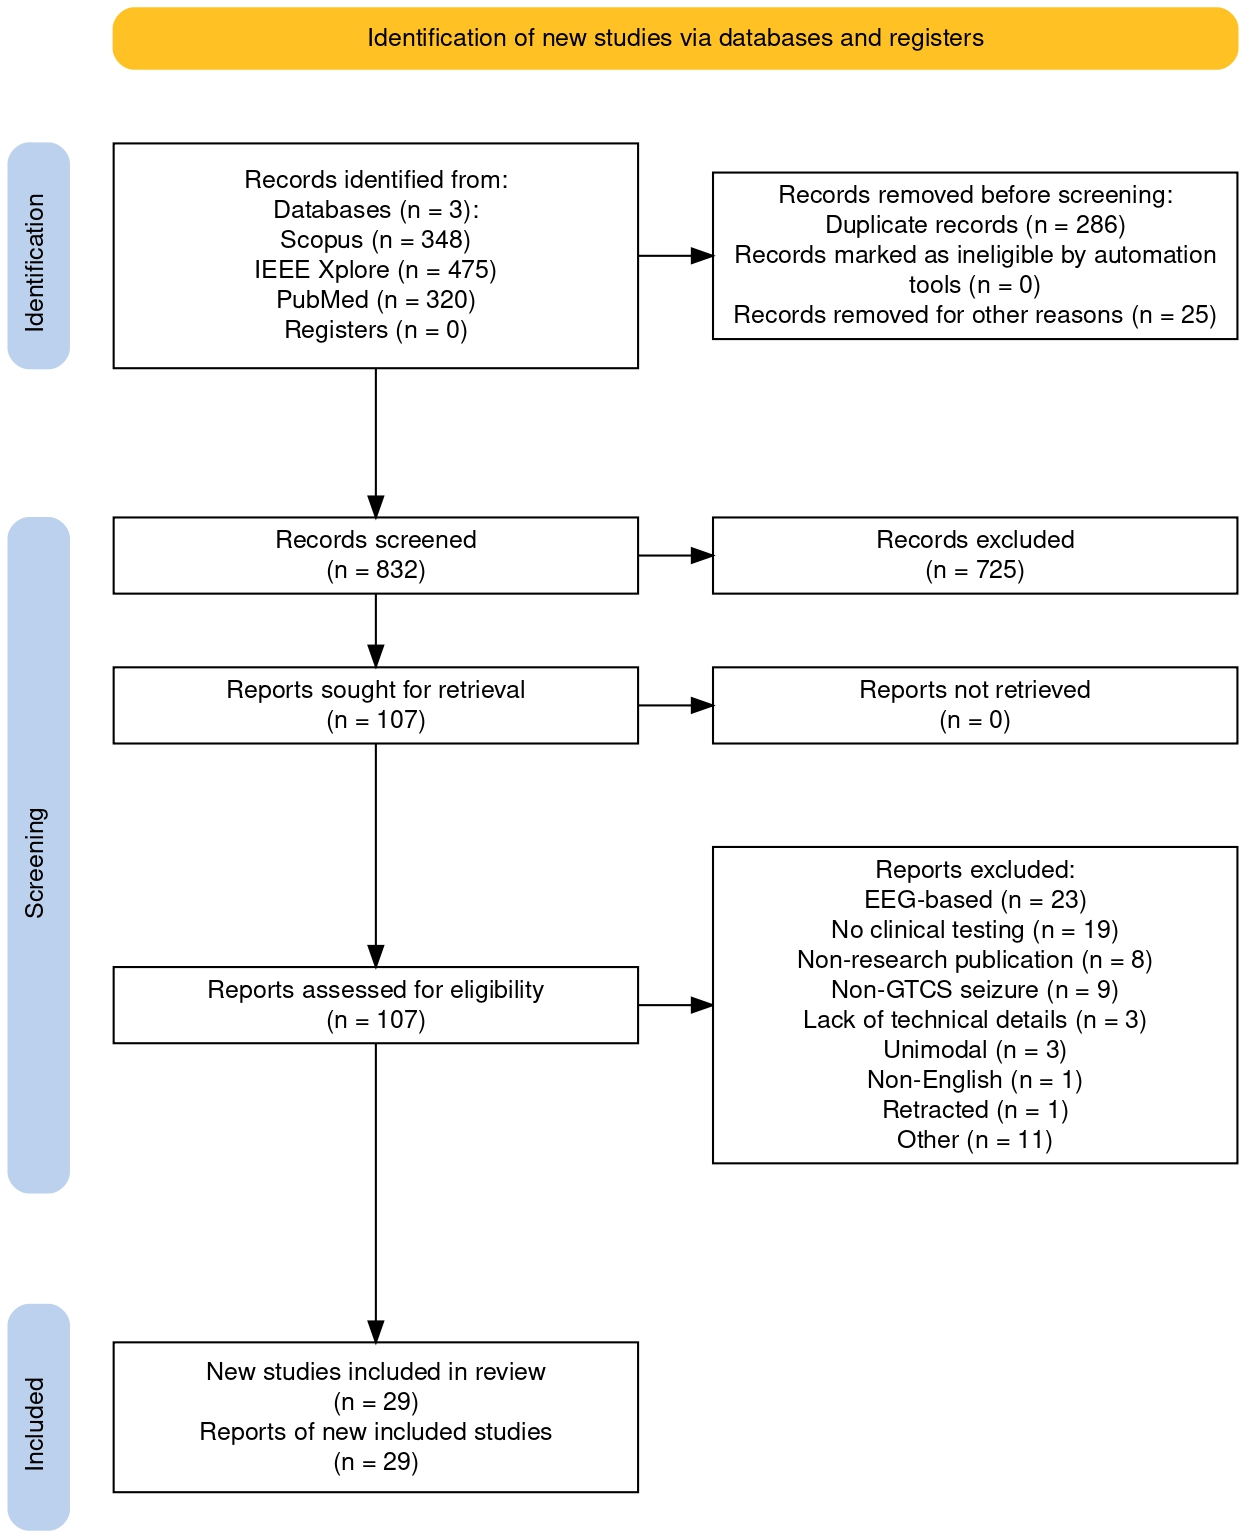
\includegraphics[width=1\textwidth]{methodology/figures/prisma_flow_diagram.jpg}
    \caption{PRISMA Flow Diagram}
    \label{fig:prisma_flow_diagram}
\end{figure}

This scoping review was conducted in accordance with the PRISMA Extension for Scoping Reviews (PRISMA-ScR) guidelines (Figure \ref{fig:prisma_flow_diagram}) \cite{Tricco2018-bb}.

Conference papers and peer-reviewed articles of various study designs were included if they investigated wearable multimodal approaches for the detection or prediction of epileptic seizures. Studies were excluded if they (1) were review articles, (2) employed a unimodal detection system, (3) lacked clinical validation, or (4) targeted focal seizures only.

Three electronic databases (Scopus, IEEE Xplore, and PubMed) were searched until April 22, 2025  using Boolean operators, wildcards, and keywords relevant to epilepsy, wearable sensors, detection outcomes, and AI-based analysis. (\href{https://docs.google.com/document/d/1FJTEZIhRoBhq3tmehHFUZllaM-GqR_4c1j9waukcQow/edit?tab=t.0}{supplementary file II}). 

After duplicates removal, retrieved articles were screened first by titles and abstracts, followed by reading through the full-text. Eight reviewers independently participated as pairs in screening. Screening decisions and record management were handled using Mendeley for reference organization and Google Sheets for collaborative screening. 

Data charting was conducted in duplicate by independent reviewers using Google Sheets. No standardized or pre-piloted data extraction form was used; instead, reviewers extracted data deemed relevant to the review objectives based on team consensus. The following variables were systematically extracted from each included study: year of publication; task type (detection, prediction, or forecasting); study characteristics (clinical setting,  average patient age, dataset size, targeted seizure types, and reference standard); device characteristics (wearability, commercial device name if applicable, and sensor placement); signal characteristics (sensor modalities, extracted biomarkers, and preprocessing steps); algorithm characteristics (task type, real-time applicability, patient-specific versus generalized model, and best-performing algorithm); and reported outcomes (performance metrics and key findings). 

Extracted data were synthesized and presented using structured tables (\href{https://docs.google.com/spreadsheets/d/1FjxwkHFbNDM84nuqg513gR_0vIVql-evoT1EMiqSYZU/edit?pli=1&gid=1255223968#gid=1255223968}{Table S1}, \href{https://docs.google.com/spreadsheets/d/1FjxwkHFbNDM84nuqg513gR_0vIVql-evoT1EMiqSYZU/edit?pli=1&gid=97270185#gid=97270185}{Table S2}).
Discrepancies during screening and data charting were resolved through collaborative discussion.


\section{Results}

A total of 35 studies were included in this review (Table number). These studies utilized a range of devices for seizure detection, including both commercial and non-commercial options. The most frequently used commercial device was the EMPATICA E4, featured in 7 studies [studies references]. Additional studies employed either laboratory-developed devices or other commercial devices, such as: Shimmer, Samsung SM-R800 watch, Microsoft wristband, and iCalm watch.

All included studies assessed various combinations of the following physiological and movement modalities: Accelerometer (ACC), Blood Volume Pulse (BVP), Gyroscope (Gyro), Electromyography (EMG), Heart rate (HR), Oxygen Saturation (SPO2), Electrodermal activity (EDA), electrocardiography (ECG), temperature, and Heart rate variability (HRV).

\subsection{Demographics}

Of the studies reviewed, 25 were conducted exclusively in inpatient settings. One study didn’t explicitly state the setting, but it is implied for home monitoring \cite{Hassan2022-do}. 2 studies included data from both inpatient and outpatient environments \cite{Regalia2019-ch, Nasseri2021-xn}. Sample sizes varied widely, ranging from as few as 4 \cite{Li2022-ty} to as many as 166 \cite{Yu2023-ss} participants. Five studies focused solely on adults aged 18 \cite{Gharbi2024-ad} to 64 \cite{Cogan2017-lg} years, with one additional adult study not specifying the age range \cite{Bottcher2021-zl}, and 1 providing the mean age only \cite{Hamlin2021-sd}. Ten studies were conducted exclusively in pediatric populations, including two that did not specify exact ages but stated that participants were children \cite{Milosevic2016-ee, De_Cooman2018-pq}. Twelve studies included mixed-age populations, with ages spanning from 2 \cite{Van_Andel2017-yx} to 75 \cite{Larsen2024-vn} years, including three that didn’t specify the age range \cite{Nasseri2021-xn, Regalia2019-ch, Xu2022-tx}. Six studies did not provide any information about the participants' ages. Additionally, three studies included healthy participants to test the performance of their seizure detection methods \cite{Wang2022-lt, Larsen2024-vn, Wang2025-my}.

\subsection{Modalities}

% \setlength{\tabcolsep}{12pt} 

\begin{table}
    \caption{Modalities (Detection)}
    \vspace{1em}
    \label{tab:modalities}
    \footnotesize
\begin{tabularx}{\textwidth}{@{}lCCCC@{}}
\toprule
\thead{Modality} & \thead{Sensitivity} & \thead{FAR/24H} & \thead{Accuracy} & \thead{Studies} \\
\midrule
ACC, GYR, sEMG, EDA & [81.69\%--95.24\%] & [0.64--1.21] & [93.16\%--96.81\%] & \cite{Wang2025-ql, Ge2023-ab, Li2022-ty, Wu2024-yl, Wang2022-lt} \\
ACC, PPG & [80\%--86\%] & [0.2609--13.63] & --- & \cite{Ali2020-ke, Tang2021-td, Arends2018-ew, Yu2023-ss} \\
ACC, EDA, PPG & [93\%--100\%] & [0.08--2.339] & --- & \cite{Xu2022-tx, Nasseri2021-xn} \\
ACC, ECG & [87\%--92\%] & --- & --- & \cite{Van_Andel2017-yx, Hegarty-Craver2021-hk} \\
ACC, GYR & [76.84\%--96\%] & [0.98] & [97.28\%] & \cite{Larsen2024-vn, Dong2022-oo} \\
ACC, GYR, sEMG & [97\%--100\%] & --- & --- & \cite{Wang2025-my, Gheryani2017-yg} \\
ACC, sEMG & [90.91\%] & --- & --- & \cite{Milosevic2016-ee} \\
ACC, EDA & [93.9\%--97.2\%] & [0.53--1.8] & [96.7\%] & \cite{Regalia2019-ch, Poh2012-af, Chowdhury2022-bi} \\
ACC, ECG, sEMG & [90.9\%] & --- & --- & \cite{De_Cooman2018-pq} \\
ACC, ECG, EDA, sEMG & --- & --- & --- & \cite{Hamlin2021-sd} \\
ACC, GYR, PPG & [87\%] & [0.21] & [93\%] & \cite{Vakilna2024-hk} \\
ACC, EDA, GYR, PPG & [89\%] & [0.54] & --- & \cite{Jiang2022-zu} \\
EDA, PPG & [100\%] & --- & --- & \cite{Cogan2017-lg} \\
\bottomrule
\end{tabularx}

\end{table}

\begin{figure}
    \centering
    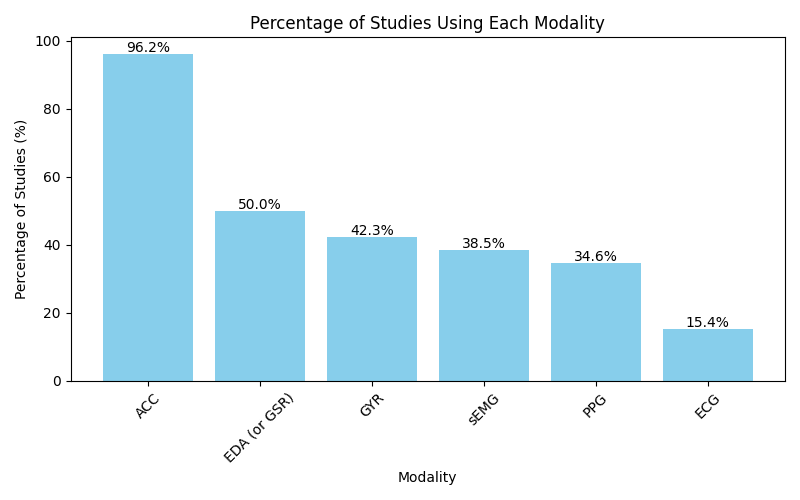
\includegraphics[width=1\textwidth]{Results/figures/percentage_of_studies_using_each_modality.png}
    \caption{Percentage of Studies Using Each Modality. Please note that studies used multiple sensors, however, the combination is not shown in this graph}
    \label{fig:percentage_of_studies_using_each_modality}
\end{figure}

\begin{figure}
    \centering
    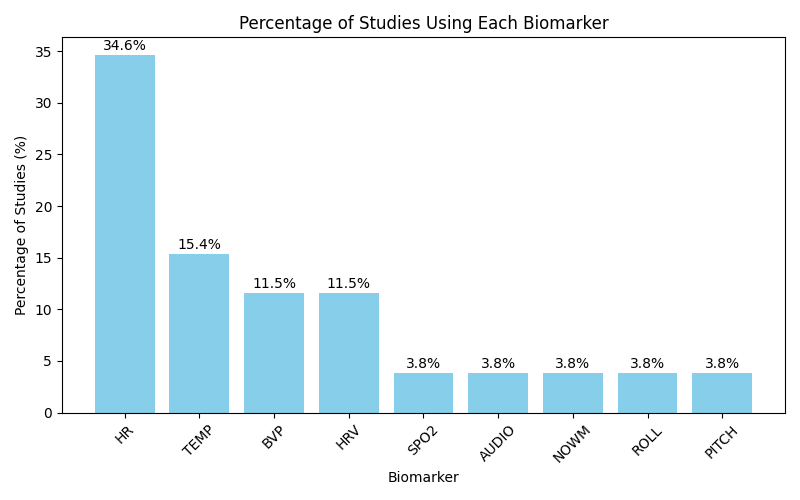
\includegraphics[width=1\textwidth]{Results/figures/percentage_of_studies_using_each_biomarker.png}
    \caption{Percentage of Studies Using Each Biomarker}
    \label{fig:percentage_of_studies_using_each_biomarker}
\end{figure}

\begin{figure}
    \centering
    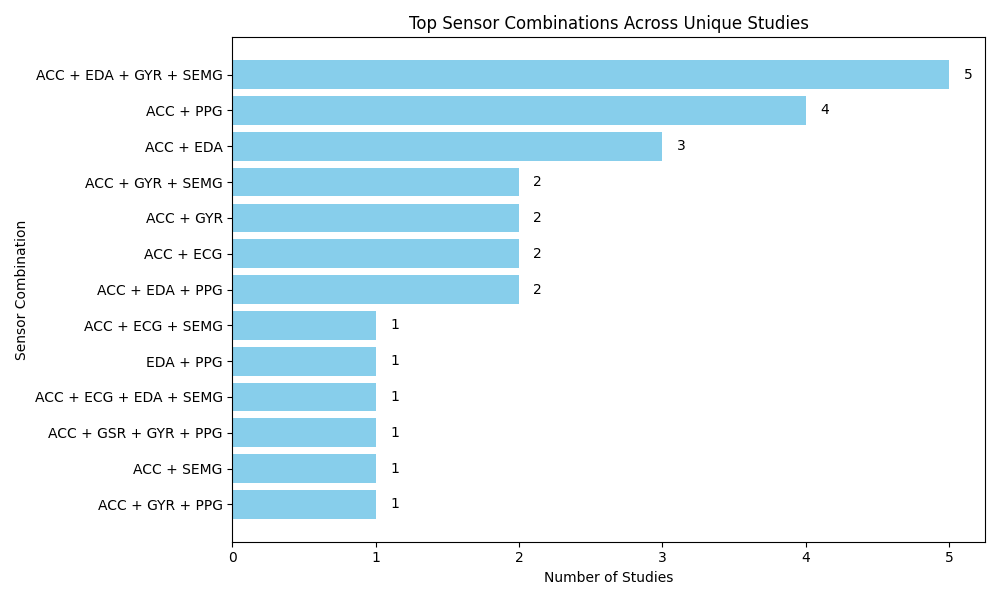
\includegraphics[width=1\textwidth]{Results/figures/freq_of_each_sensor_comp.png}
    \caption{Frequency of Each Sensor Combination}
    \label{fig:freq_of_each_sensor_comp}
\end{figure}

\subsubsection{Detection}
Among the 26 reviewed detection studies, ACC was by far the most frequently used modality (96.2\%) to capture the convulsive motor activity associated with tonic-clonic seizures. EDA followed as the second most used modality, appearing in half of the studies, while ECG was the least commonly used (15.4\%) (Figure \ref{fig:percentage_of_studies_using_each_modality}).

Several studies went beyond raw sensor signals and extracted specific biomarkers such as HR, HRV, BVP, and SpO$_2$, which were then used as features in seizure detection models. HR was the most commonly used biomarker (34.6\%), while SpO$_2$, audio, NOWM, and pitch and roll motion were each used in only 3.8\% of the studies (Figure \ref{fig:percentage_of_studies_using_each_biomarker}).

Altogether, 13 different multimodal sensor combinations were reported. The most common was ACC + GYR + sEMG + EDA (19.2\%; Figure \ref{fig:freq_of_each_sensor_comp}). Almost all studies that directly compared unimodal and multimodal systems \cite{Yu2023-ss,Milosevic2016-ee,De_Cooman2018-pq,Chowdhury2022-bi,Ge2023-ab, Wang2025-my,Tang2021-td,Li2022-ty,Hegarty-Craver2021-hk,Poh2012-af,Hamlin2021-sd,Wu2024-yl} found that multimodal systems outperformed unimodal ones. The only exception was \cite{Hegarty-Craver2021-hk}, where a cardiac algorithm using ECG alone achieved a lower FPR (1 per day) compared to ACC + ECG (2 per day).

The most commonly used multimodal sensor combination, ACC + GYR + sEMG + EDA \cite{Wang2025-ql, Ge2023-ab, Li2022-ty, Wu2024-yl, Wang2022-lt} consistently achieved high performance, with the highest reported in \cite{Wu2024-yl}. Among these studies, Wang et al. \cite{Wang2025-ql} investigated the use of derived biomarkers (PITCH and ROLL, extracted from ACC and GYR) instead of or in combination with raw ACC and GYR data. They found that substituting ACC with PITCH or ROLL improved performance across all models, with the best results obtained using SVM (Accuracy: 95.7\%, Precision: 95.7\%, Recall: 93.8\%; for ROLL: Accuracy: 95.2\%, Precision: 95.7\%, Recall: 92.5\%) compared to the original combination which achieved an accuracy of 93.4\%, precision of 95.8\%, and recall of 90.9\%. 

Another widely used combination was ACC + PPG \cite{Ali2020-ke, Tang2021-td, Arends2018-ew, Yu2023-ss}. Yu et al. \cite{Yu2023-ss} reported that for generalized motor seizures, ACC + BVP achieved the best performance with a mean AUC-ROC of 0.805, while EDA had the lowest mean AUC-ROC of 0.513. For tonic–clonic seizures, ACC alone achieved the best performance, with an AUC-ROC of 0.973, a sensitivity of 95\%, and FPR of 6.2\%. Similarly, Tang et al. \cite{Tang2021-td} reported that when ACC data was used alone, this model performed best for tonic-clonic seizures with an AUC-ROC of 0.995, however, for seizure type agnostic, ACC + BVP fusion performed best, with an AUC-ROC of 0.752. Another study \cite{Arends2018-ew}, an in-home nocturnal cohort study, reported that their sensitivity was significantly high (median 85\%) compared to a rhythmic movement-based bed sensor (median 21\%). They further analyzed feature contributions and showed that HR was the critical modality for true positives (92\%) and also for false positives, while ACC contributed only 8\% of true positives and caused no false alarms.

ACC + EDA was also one of the top and high achieving combinations \cite{Regalia2019-ch, Poh2012-af, Chowdhury2022-bi} with the highest sensitivity (97.2\%) reported by \cite{Chowdhury2022-bi} and the lowest FAR/24h (0.53) reported by \cite{Regalia2019-ch}, which validated Empatica multimodal wristbands (E4 and Embrace) as reliable tools for GTCS detection in real-world and Epilepsy Monitoring Units (EMUs) settings. Chowdhury et al. \cite{Chowdhury2022-bi} reported that fusing ACC and EDA significantly improved classification accuracy (96.7\%) and reduced FAR (unspecified) compared to unimodal approaches. Similarly, Poh et al. \cite{Poh2012-af} reported that the overall performance was lower when only ACC features were included.

While most studies incorporate both physiological and motion-based sensors in their sensor suite, 19.2\% of the studies were purely motion-based, using sensor combinations of ACC + GYR \cite{Larsen2024-vn, Dong2022-oo}, ACC + GYR + sEMG \cite{Wang2025-my, Gheryani2017-yg} and ACC + sEMG \cite{Milosevic2016-ee}. Among these, the ACC + sEMG + GYR configuration achieved the best performance. In addition to studying their significance in seizure detection, a few studies have tested for the optimal sensor placement \cite{Milosevic2016-ee, De_Cooman2018-pq}, showing that using sensors on different body locations can reduce false alarms and improve performance. \cite{Milosevic2016-ee} identified the left wrist (generally the non-dominant hand) and right ankle as optimal positions for ACC sensors, while bilateral biceps were optimal for sEMG. 

For details of the remaining reported combinations, refer to the Modality Table.

\subsubsection{Prediction and Forecasting}
All three studies used EDA and PPG in their sensor suite. One seizure forecasting study additionally used ACC \cite{Meisel2020-ii}. PPG was used to extract biomarkers like HR in \cite{Vieluf2023-ta, Vieluf2023-zv}, HRV in \cite{Vieluf2023-zv}, and BVP in \cite{Meisel2020-ii}. TEMP was also among the biomarkers used by \cite{Vieluf2023-zv, Meisel2020-ii}, however in \cite{Vieluf2023-zv}, TEMP did not differ between seizure and non-seizure groups and was therefore not included in further analysis. Vieluf et al. \cite{Vieluf2023-ta, Vieluf2023-zv} identified EDA and HR as containing sufficient seizure-predictive information, with reported performance of 62\% sensitivity and an accuracy range of 68–68.89\%. These findings were further supported in \cite{Vieluf2023-zv}, where HRV was additionally shown to carry predictive value: patients with an impending seizure had lower HR and higher HRV compared to seizure-free patients in evening recordings. In \cite{Meisel2020-ii}, forecasting performance was highest when all modalities (EDA, BVP, TEMP, ACC) were combined achieving significant seizure forecasting (better-than-chance) in 43\% of patients (30/69), where the mean sensitivity was 75.6\%, the mean time in warning (TiW) was 47.2\% and the mean prediction horizon was 31.6 minutes. Each modality contributed uniquely, though accelerometry sometimes reduced performance in low-performing patients.



\subsection{Preprocessing}

\subsubsection{Signal Synchronization and Quality Control}
To match biosignal recordings with reference data like EEG or video, many studies performed time synchronization. This included adjusting for time drift between devices using start and end timestamps or using the network time protocol (NTP) \cite{Onorati2017-bn,Vakilna2024-hk,Tang2021-td}. Some studies checked signal quality and removed invalid parts of the data. For example, segments were excluded if the temperature was too low or too high (less than 27°C or more than 45°C), which indicated the device was not worn properly \cite{Yu2023-ss,Tang2021-td}. Other signals were removed based on quality checks, like low EDA amplitude or poor PPG quality \cite{Ge2023-ab,Arends2018-ew}. Also, the first and last 15 minutes of recordings were sometimes discarded to avoid artifacts from calibration \cite{Yu2023-ss}.

\subsubsection{Noise and Artifact Removal}
Most studies used filtering to reduce unwanted signals caused by movement, other physiological activity, or environmental noise. Bandpass filters were common. For example, accelerometer and gyroscope signals were filtered between 0.2–47 Hz \cite{Milosevic2016-ee,De_Cooman2018-pq}, 1–24 Hz \cite{Wu2024-yl}, or 0.5–35 Hz \cite{Gheryani2017-yg}. EMG signals were filtered between 20–90 Hz \cite{Wu2024-yl} or with a high-pass filter at 20 Hz \cite{Milosevic2016-ee,De_Cooman2018-pq}. ECG signals used a notch filter at 60 Hz to remove electrical interference from power lines \cite{Hamlin2021-sd}. Some studies smoothed signals using moving averages, like a 10-minute average for temperature \cite{Yu2023-ss} or a 15-point average for EDA \cite{Wang2022-lt}. Median filters were also used for EDA signals \cite{Wang2025-ql}. A few studies used wavelet transforms to break down signals like ECG-derived respiration (EDR) to level 7 to improve entropy \cite{Forooghifar2022-dm}, or to clean heart rate and GSR signals \cite{Jiang2022-zu}.

\subsubsection{Data Segmentation and Windowing}
To analyze the signals, the data was divided into short or long windows. The window length depended on the type of seizure being studied. Short windows, between 2 and 10 seconds, were used to detect convulsive seizures. For example, one study used 2-second windows with 75\% overlap for ACC and EMG data \cite{Milosevic2016-ee,De_Cooman2018-pq,Poh2012-af}. Longer windows, from 1 to 7 minutes, were used to detect slower changes in the body, such as with PPG, EDA \cite{Ramirez-Peralta2021-nq}, HRV \cite{Jiang2022-zu}, or for detecting generalized convulsive seizures (GCS) \cite{Vakilna2024-hk}. Some studies removed low-motion periods by checking if acceleration was too low, such as standard deviation below 0.2g \cite{Wang2022-lt,Dong2022-oo}, or only analyzed data when acceleration was above 0.1g \cite{Larsen2024-vn}.

\subsubsection{Class Imbalance Handling}
Since seizures are rare compared to non-seizure events, many studies dealt with this class imbalance. One method was undersampling, where non-seizure data was randomly removed to create a more balanced dataset. For example, one study used a seizure-to-nonseizure ratio of 1:1.5 \cite{Yu2023-ss,Tang2021-td}. Other studies used oversampling, where seizure data was repeated to make it more balanced, especially for short seizures \cite{Larsen2024-vn}. Some used automatic filtering to remove non-seizure data based on certain signal patterns, like when the main frequency of acceleration was below 2 Hz or when the signal had a noncross ratio above 0.9 \cite{Wang2022-lt}.

\subsubsection{Features Extraction}
Most studies created features from the signals to use in machine learning models. Time-domain features included basic statistics like mean, variance, and entropy \cite{Wang2022-lt,Dong2022-oo}, zero-crossing rates \cite{De_Cooman2018-pq}, and counts of local maxima \cite{Milosevic2016-ee}. Frequency-domain features included power in certain frequency bands, like 9–22.5 Hz \cite{Milosevic2016-ee}, FFT peaks \cite{Wang2022-lt}, and heart rate variability from Lomb-Scargle analysis \cite{Ramirez-Peralta2021-nq}. Some studies combined features from different sensors, such as ACC and EDA \cite{Regalia2019-ch,Wu2024-yl}, or used decision-level fusion \cite{Chowdhury2022-bi}. To reduce the number of features and keep only the most useful ones, they used methods like minimum redundancy maximum relevance (mRMR) \cite{Wang2022-lt,Ge2023-ab}, ANOVA \cite{Dong2022-oo}, or the Wilcoxon rank-sum test \cite{Vakilna2024-hk}.

\subsubsection{Normalization and Baseline Correction}
Normalization helped make signals more comparable between different people or recording sessions. Some studies used z-score normalization, which adjusts signals to have a mean of zero and a standard deviation of one \cite{Nasseri2021-xn}. Others used moving baselines, where the recent history of a signal (such as over 60 seconds) was used to calculate thresholds for heart rate or oxygen saturation \cite{Cogan2015-lu}. Personalized baselines were also used, where each subject’s median signal was used as a reference point \cite{Jiang2022-zu}.


\subsection{Algorithms}

\subsubsection{Deep Learning Methods}
Studies have leveraged deep learning architectures to automatically learn hierarchical features and model complex temporal dependencies in multimodal sensor data. Deep learning methods were employed in 19.2\% of the reviewed detection studies (Table \ref{tab:deep_and_personalized_algos}) \cite{Yu2023-ss, Nasseri2021-xn, Larsen2024-vn, Wang2025-ql, Tang2021-td} and in 66.7\% of the prediction studies (Table \ref{tab:prediction_modalities_and_algos}) \cite{Vieluf2023-ta, Meisel2020-ii}. The most prominent architectures included Convolutional Neural Networks (CNNs) \cite{Yu2023-ss, Tang2021-td}, Long Short-Term Memory (LSTM) networks \cite{Meisel2020-ii, Yu2023-ss, Wang2025-ql}, and hybrid models combining both \cite{Yu2023-ss}.

For the seizure detection task, hybrid CNN-LSTM models were shown to be particularly effective. One study identified a CNN-LSTM fusion model using accelerometer (ACC) and blood volume pulse (BVP) data as the best overall algorithm, achieving 83.9\% sensitivity and a detection delay of 28 seconds across 28 seizure types \cite{Yu2023-ss}. For generalized tonic-clonic (GTC) seizures specifically, this model reached 95\% sensitivity \cite{Yu2023-ss}. Standalone LSTM networks were also successfully applied, particularly for their ability to capture time-series dynamics. One such study demonstrated that an LSTM model with transfer learning significantly outperformed traditional learning, achieving 93\% sensitivity for in-hospital motor seizures with a false alarm rate (FAR) of 2.3 per day \cite{Nasseri2021-xn}. Another study utilized an LSTM with attitude angle signals, among others, to achieve an accuracy of 83.4\% \cite{Wang2025-ql}.

Other neural network architectures were also explored. A CNN-based model was found to be feasible for detecting a broad variety of seizure types using ACC and BVP signals \cite{Tang2021-td}. Simpler Artificial Neural Networks (ANNs) also proved effective, with one study reporting 100\% sensitivity in detecting nocturnal tonic seizures in an independent test set \cite{Larsen2024-vn}. In the context of personalization, an autoencoder model achieved 100\% sensitivity for GTC seizures in select patients, although it was noted to be less scalable \cite{Yu2023-ss}.

For the forecasting and prediction tasks, one study \cite{Meisel2020-ii} employed LSTM neural networks trained using leave-one-subject-out cross-validation on continuously collected retrospective data. Another study \cite{Vieluf2023-ta} selected Deep Canonically Correlated Autoencoders (DCCAE) for training and validation, testing three different architectures: Fully Connected DCCAE (FC-DCCAE), Convolutional Neural Network DCCAE (CNN-DCCAE), and Gated Recurrent Unit DCCAE (GRU-DCCAE). Among these, GRU-DCCAE yielded the best clustering accuracy of 68.89\%. Both studies lacked real-time implementation, relying instead on retrospective or offline data analysis.


\subsubsection{Ensemble Methods}
Ensemble learning, which combines multiple machine learning models to improve predictive performance, was a prominent and effective strategy in several detection studies (Table \ref{tab:ensemble_algos}). Ensemble classifiers were used in 23\% of the detection studies  including bagging, boosting, and more complex stacked architectures \cite{Wang2022-lt, Chowdhury2022-bi, Vakilna2024-hk, Dong2022-oo, Jiang2022-zu, Wu2024-yl}. Also, one forecasting study reported the use of random forest (RF) classifier \cite{Vieluf2023-zv}.

For the seizure detection task, bagging-based methods, such as Random Forest (RF) and Bagged Decision Trees, were particularly common \cite{Chowdhury2022-bi, Wang2022-lt, Wu2024-yl, Vakilna2024-hk}. One study demonstrated that  algorithm achieved 90\% sensitivity with a low false alarm rate of 1.21 per 24 hours for tonic-clonic seizures in a daily setting \cite{Wang2022-lt}. Another study found that a Bagged Decision Tree classifier, when applied to fused accelerometer (ACC) and electrodermal activity (EDA) data, yielded GTCS detection accuracy of 96.7\% \cite{Chowdhury2022-bi}.

A more advanced approach was the Two-Layer Ensemble Method (TLEM), which stacked multiple base learners including RF, Extra Trees (ET), Gradient Boosting Decision Tree (GBDT), and AdaBoost (ADB) \cite{Dong2022-oo}. This stacked model was shown to outperform all of its single-layer components, achieving a particularly high sensitivity of 94.57\% and a FAR of 0.46 per 24 hours for nocturnal seizures. While achieving a sensitivity of 76.84\% and a FAR of 0.98 per 24 hours for overall, day and night, seizures \cite{Dong2022-oo}.

For the seizure forecasting task (Table \ref{tab:prediction_modalities_and_algos}), Vieluf et al. \cite{Vieluf2023-zv} evaluated the performance of seven supervised learning algorithms with RF achieving the higher accuracy of 68\% and sensitivity of 62\%.


\subsubsection{Traditional Machine Learning}
In detection, 30.8\% of the studies reported the successful application of models such as SVM, K-Nearest Neighbors (KNN), and Linear Discriminant Analysis (LDA) (Table \ref{tab:trad_ml_algos})\cite{Milosevic2016-ee, Hamlin2021-sd, Poh2012-af, Ge2023-ab, Li2022-ty, Xu2022-tx, Wang2025-my, De_Cooman2018-pq}.

The most frequently and successfully implemented classifier was SVM \cite{Milosevic2016-ee, De_Cooman2018-pq, Poh2012-af, Ge2023-ab, Li2022-ty, Xu2022-tx, Wang2025-my}. One study found that an SVM delivered the best trade-off between accuracy and false alarms, achieving a 100\% accurate recognition rate with just 0.08 false alarms per day \cite{Xu2022-tx}. Another study concluded that a linear SVM (SVM-L) provided the optimal sensitivity and overall performance among several tested models, achieving sensitivity of 100\% and FAR/24h of 0.107 \cite{Wang2025-my}. Other studies reported SVM sensitivities ranging from 81.7\% \cite{Li2022-ty} to 90.01\% \cite{Milosevic2016-ee}. The effectiveness of SVMs was also noted when using attitude angle signals, where they yielded the highest overall accuracy compared to decision trees and LDA \cite{Wang2025-ql}.

Other traditional classifiers also showed strong performance. KNN, particularly when using a cosine distance metric on features from four combined modalities, achieved a high sensitivity of 88.16\% and accuracy of 93.16\% \cite{Ge2023-ab}. LDA was also utilized, with one study reporting and AUC-ROC of 0.914 \cite{Hamlin2021-sd}.


\subsubsection{Rule-based and Threshold-based Methods}
These methods rely on predefined physiological patterns or thresholds to trigger a seizure detection. This approach was used in 19.2\% of the reviewed detection studies (Table \ref{tab:rule_based_algos}) \cite{Cogan2017-lg, Ali2020-ke, Hegarty-Craver2021-hk, Gheryani2017-yg, Arends2018-ew}.

One study developed a system based on a multi-biosignal pattern, defining a seizure event as a sequence of HR increase, followed by a decrease in SpO$_2$, and a subsequent rise in electrodermal activity \cite{Cogan2017-lg}. This rule-based method achieved an accuracy of 100\% for seizure detection in GTCS patients \cite{Cogan2017-lg}. Another study implemented a system with decision rules based on three factors: shaking, from an ACC, HR, and TEMP \cite{Ali2020-ke}. By classifying risk into discrete levels, the system achieved a sensitivity of 85\% \cite{Ali2020-ke}. 

A threshold-based algorithm using cardiac physiological features was also reported, detecting 92\% of seizures with tonic/clonic movements \cite{Hegarty-Craver2021-hk}. Another approach applied a Shewhart control chart with exponentially weighted moving averages to motion inertial and muscular activity, achieving a 97\% detection rate with a 4\% FAR \cite{Gheryani2017-yg}. A further study employed a combined accelerometry and heart rate threshold algorithm in a residential care setting, reaching a median sensitivity of 86\% with a positive predictive value (PPV) of 49\% \cite{Arends2018-ew}.


\subsubsection{Methods with Personalization}
Recognizing the high degree of inter-patient variability in seizure manifestation, many studies investigated or recommended personalized algorithms. For detection studies, 30.8\% highlighted the benefits of tailoring models to individual patients (Table \ref{tab:deep_and_personalized_algos}) \cite{Yu2023-ss, Poh2012-af, Nasseri2021-xn, Milosevic2016-ee, Hamlin2021-sd, Jiang2022-zu, Hegarty-Craver2021-hk, Wang2025-ql}.

One study showed that a "semi-patient-specific" approach, which included prior seizure examples from the test patient in the training data, improved sensitivity from 88\% to 94\% compared to a generic model \cite{Poh2012-af}. Similarly, a personalized autoencoder was able to achieve 100\% sensitivity for GTC seizures in certain individuals, a level of performance not reached by the generalized model \cite{Yu2023-ss}. A particularly effective technique was transfer learning, where a pre-trained general model was fine-tuned on patient-specific data. This method significantly improved performance, reducing the FAR from 11.3 per day with traditional learning to 2.33 per day \cite{Nasseri2021-xn}.

Other studies underscored the need for personalization by observing that false alarms and key predictive features varied significantly between individuals \cite{Milosevic2016-ee, Hamlin2021-sd}. Some methodologies were inherently personalized, such as a system that tracked individual "physiomes" by establishing personal physiological baselines to detect seizure-related deviations \cite{Jiang2022-zu}.

\begin{table}
    \footnotesize
    \caption{Algorithms (Detection)}
    \label{tab:algos}
%%%%%%%%%%%%%%%%%%%%%%%%%%%%%%%%%%%%%%%%%%%%%
%% Deep Learning and personalized methods
%%%%%%%%%%%%%%%%%%%%%%%%%%%%%%%%%%%%%%%%%%%%%
\begin{subtable}{\textwidth}

\caption{Deep Learning and Personalized Algorithms}
\label{tab:deep_and_personalized_algos}

\begin{tabularx}{\textwidth}{@{}lCCCCC@{}}
\toprule
\thead{Algorithm} & \thead{Studies} & \thead{Real-time\\Analysis} & \thead{Sensitivity} & \thead{FAR} & \thead{AUC-ROC} \\
\midrule
\multirow{2}{*}{CNN} & \cite{Yu2023-ss} & \multirow{2}{*}{No} & 95\% & --- & 0.769 \\ 
% \cline{2-2}\cline{4-6}
 & \cite{Tang2021-td} &  & 80\% & 13.63/24h & 0.752 \\ 
\midrule
CNN + LSTM & \cite{Yu2023-ss} & No & 83.9\% & --- & 0.789 \\ 
\midrule 
LSTM & \cite{Wang2025-ql} & Yes & --- & 8.46/24h & --- \\ 
\midrule
ANN & \cite{Larsen2024-vn} & No & 96\% & 0.23/Night & --- \\ 
\midrule
Transfer Learning$^a$ & \cite{Nasseri2021-xn} & --- & 67\% & 4.8/24h & 0.97 \\
\midrule
Personalized Autoencoder$^a$ & \cite{Yu2023-ss} & No & 100\% & [0.0--95.36]/24h & --- \\
\bottomrule
\end{tabularx}

\vspace{0.5em}

All are inpatient studies.

$^a$Algorithms with personalization.

\vspace{1em}

\end{subtable}

%%%%%%%%%%%%%%%%%%%%%%%%%%%%%%%%%%%%%%%%%%%%%
%% Ensemble Methods
%%%%%%%%%%%%%%%%%%%%%%%%%%%%%%%%%%%%%%%%%%%%%
\begin{subtable}{\textwidth}

\caption{Ensemble Algorithms}
\label{tab:ensemble_algos}

\begin{tabularx}{\textwidth}{@{}CCCCCCC@{}}
\toprule
\thead{Algorithm} & \thead{Studies} & \thead{Inpatient/\\Outpatient} & \thead{Real-Time\\Analysis} & \thead{Sensitivity} & \thead{FAR/24h} & \thead{Accuracy} \\
\midrule
\multirow{2}{*}{Random Forest} & \cite{Wang2022-lt} & Outpatient & \multirow{2}{*}{No} & 90\% & 1.21 & --- \\
 & \cite{Vakilna2024-hk} & Inpatient &  & 87\% & 0.21 & 93\% \\
\midrule
Bagged decision Tree Classifier & \cite{Chowdhury2022-bi} & Outpatient & Yes & --- & --- & 95.1\% \\
\midrule
XGBoost & \cite{Jiang2022-zu} & Inpatient & Yes & 80\% & 1.1 & --- \\
\midrule
\multirow{2}{*}{}{Two-Layer Ensemble Model} & \multirow{2}{*}{\cite{Dong2022-oo}} & \multirow{2}{*}{Outpatient} & \multirow{2}{*}{No} & 76.84\% (Overall) & 0.98 (Overall) & 97.28\% (Overall) \\
 &  &  &  & 94.57\% (Overall) & 0.46 (Night) & 91.37\% (Night) \\
\bottomrule
\end{tabularx}
\end{subtable}


\end{table}

%%%%%%%%%%%%%%%%%%%%%%%%%%%%%%%%%%%%%%%%%%%%%
%%%%%%%%%%%%%%%%%%%%%%%%%%%%%%%%%%%%%%%%%%%%%
%%%%%%%%%%%%%%%%%%%%%%%%%%%%%%%%%%%%%%%%%%%%%

\begin{table}
    \footnotesize
    \ContinuedFloat
    \caption{Algorithms (Detection) cont.}
    \label{tab:algos_cont}
    
%%%%%%%%%%%%%%%%%%%%%%%%%%%%%%%%%%%%%%%%%%%%%
%% Traditional Machine Learning
%%%%%%%%%%%%%%%%%%%%%%%%%%%%%%%%%%%%%%%%%%%%%
\vspace{1em}
\begin{subtable}{\textwidth}
    \caption{Traditional Machine Learning Algorithms}
    \label{tab:trad_ml_algos}
\begin{tabularx}{\textwidth}{@{}CCCCCCC@{}}
\toprule
\thead{Algorithm} & \thead{Studies} & \thead{Real-Time\\Analysis} & \thead{Sensitivity} & \thead{FAR/24h} & \thead{Accuracy} & \thead{AUC-ROC} \\ \midrule
\multirow{6}{*}{SVM} & \cite{Poh2012-af} & No & 88\% & 1.0 & --- & --- \\
 & \cite{Ge2023-ab} & No & 87.13\% & --- & --- & --- \\
 & \cite{Xu2022-tx} & Yes & --- & 0.08 & 100\% & --- \\
 & \cite{Wang2025-my} & No & 100\% & 0.107 & --- & --- \\
 & \cite{Li2022-ty} & No & 81.7\% & 0.64 & --- &  \\
 & \cite{Milosevic2016-ee} & No & 90.01\% & --- & --- & --- \\
\midrule
KNN & \cite{Ge2023-ab} & No & 88.16\% & --- & 93.16\% & --- \\
\midrule
LDA & \cite{Hamlin2021-sd} & No & --- & --- & --- & 0.914 \\ \bottomrule
\end{tabularx}

\vspace{0.5em}

All are inpatient studies.

\end{subtable}

%%%%%%%%%%%%%%%%%%%%%%%%%%%%%%%%%%%%%%%%%%%%%
%% Rule-Based
%%%%%%%%%%%%%%%%%%%%%%%%%%%%%%%%%%%%%%%%%%%%%
\vspace{1em}
\begin{subtable}{\textwidth}
    \caption{Rule-based and Threshold-based Algorithms}
    \label{tab:rule_based_algos}
\begin{tabularx}{\textwidth}{@{}CCCCCC@{}}
\toprule
\thead{Studies} & \thead{Real-Time\\Analysis} & \thead{Sensitivity} & \thead{FAR} & \thead{Accuracy} & \thead{AUC-ROC} \\ \midrule
\cite{Hegarty-Craver2021-hk} & Yes & 92\% & 2.09/24h & --- & --- \\
\cite{Ali2020-ke} & Yes & 85\% & 26.09\% & --- & 0.8682 \\
\cite{Arends2018-ew} & Yes & 86\% & 0.25/Night & --- & --- \\
\cite{Van_Andel2017-yx} & No & 87\% & 6.3/Night & --- & --- \\
\cite{Cogan2017-lg} & No & --- & --- & 100\% & --- \\
\cite{Gheryani2017-yg} & No & 97\% & 4\% & --- & --- \\ \bottomrule
\end{tabularx}

\vspace{0.5em}

All are inpatient studies.

\end{subtable}

\end{table}
\begin{table}
    \caption{Modalities and Algorithms For Prediction and Forecasting}
    \label{tab:prediction_modalities_and_algos}
    \footnotesize
\begin{tabularx}{\textwidth}{@{}CCCCC@{}}
\toprule
Modalities & Algorithm & Accuracy & Sensitivity & Study \\ \midrule
ACC, PPG, EDA & LSTM & --- & 75.6\% & \cite{Meisel2020-ii} \\
PPG, EDA & Random Forest & 68\% & 62\% & \cite{Vieluf2023-zv} \\
PPG, EDA & GRU-DCCAE & 68.89\% & --- & \cite{Vieluf2023-ta} \\ \bottomrule
\end{tabularx}

\vspace{0.5em}

All are inpatient studies.

All studies lack real-time data analysis.

\end{table}

\section{Discussion}

\subsection{Modalities}

\begin{figure}
    \centering
    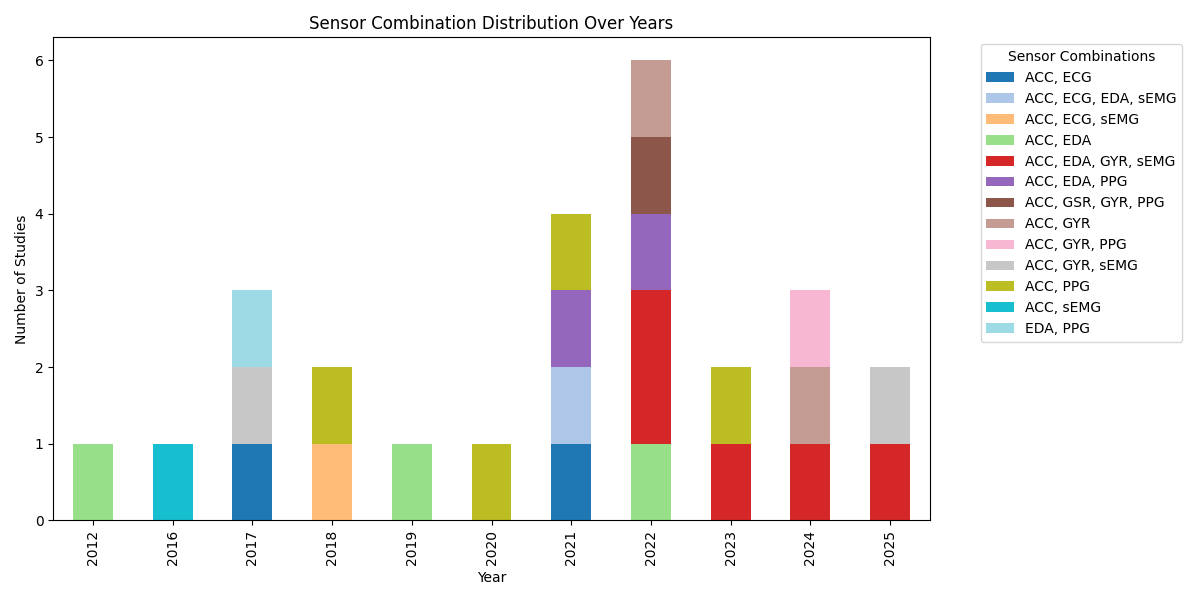
\includegraphics[width=1\textwidth]{Discussion/figures/Sensor_Combination_Distribution_Over_the_Years.png}
    \caption{Sensor combination distribution over the years.}
    \label{fig:sensor_comb_over_years}
\end{figure}

\subsubsection{Detection}
Based on the 26 reviewed articles, it is apparent that non-EEG multimodal sensor configurations for detecting motor seizures are feasible and have a great promise compared to conventional detection and management methods. 

It is important to note that direct comparison across the reviewed studies is challenging due to methodological heterogeneity, differences in study populations, and variability in training datasets. Nevertheless, the ACC + GYR + EDA + sEMG sensor combination (\textcolor{red}{Figure 5}) performance is consistently high across studies (table \ref{tab:modalities}) regardless to the study setups. This may be because these setups combine the reliability of motion-based detection through ACC, GYR, and sEMG with the stabilizing contribution of physiological signals such as EDA, which helps reduce false alarms and enhance overall performance. Additionally, sEMG has been reported to rapidly detect seizures with notably low detection delay (11.7s) [21], highlighting its importance for timely intervention.

ACC + EDA is also one of the top performing combinations, with the advantages of less sensor modalities used to indicate less costs, more easier data pre-processing and signal fusion models. This is perhaps due to EDA’s sensitivity to sympathetic activation which occurs closely with motor seizure onset consistent across multiple studies involving both children and adults [40], in addition to EDA being less sensitive to motion artifacts than other physiological signals like PPG for instance [46], making it more robust. Additionally, studies have demonstrated peri-ictal rises in EDA correlate with postictal generalized EEG suppression (PGES), a known SUDEP risk factor [2, 31], highlighting the potential of EDA in SUDEP prevention.

While this highlights the significance of EDA data in seizure detection, some studies have reported poor performance of EDA as a standalone modality and even when combined with other sensors such as PPG or ACC [1, 4]. This variability across studies stems perhaps from the age-related variability in EDA signals reported by the pediatric study [23], highlighting the need for algorithms trained on EDA to count for such variability. 

Other physiological sensors such as PPG have also been widely used to extract biomarkers including HR [15, 3, 7, 28, 9, 8], HRV [7, 8], SpO2 [15], and BVP [3, 4, 1]. Among these, BVP in particular has shown strong potential, consistently achieving high performance across seizure types. This is consistent with findings from the observational clinical study conducted by Mohammadpour Touserkani et al. [45], where not only heart rate–dependent variables (frequency), but also other features of the PPG signal such as smoothness and slope were shown to vary relative to seizure timing. These additional PPG-derived features contribute to the improved ability of BVP-based detection algorithms to accurately identify seizures beyond the sole use of heart rate metrics, highlighting the superior seizure discriminative information contained in BVP signals.

ECG has also been employed to derive HR [5, 20, 21] and HRV [20], with some studies reporting that unimodal ECG systems can achieve performance comparable to multimodal approaches [21, 20]. However, ECG w as used less frequently in the reviewed studies, largely due to its susceptibility to motion artifacts [5], its relative impracticality as a wearable sensor (requiring multiple electrodes to be placed on the chest or limbs), and the high inter-patient variability observed in cardiac-derived signals [21, 5].

Because of these limitations, ECG has mostly been used in nocturnal studies [5, 21]. This is relevant since SUDEP is more likely to happen at night [30], and HR and HRV are under investigation as potential SUDEP   biomarkers [31]. Thus, ECG may serve a dual role in seizure detection and monitoring SUDEP-related autonomic changes.

Some studies have also investigated the use of non-traditional biomarkers for seizure detection, and interestingly, several of these have demonstrated detection capabilities comparable to, or even exceeding, those of more established biomarkers. Hamlin et al. [16] investigated the incorporation of audio features, derived from a MIC, in the detection system and reported that audio signals proved to be among the top ten features establishing separability between seizure and non-seizure data in four or five patients. Wang et al. [11] investigated the incorporation of attitude angle signals  like PITCH or ROLL in their detection system and reported that in multimodal combinations, adding PITCH or ROLL alongside or replacing ACC, GYR outperformed combinations that excluded them across all models, as attitude signals were shown to have better anti-interference ability i.e. the attitude angle signals didn’t show a wide range of energy enhancements compared to ACC and GYR in non-seizure periods.  Instead of using raw ACC data, Xu et al. [28] used NOWM to distinguish seizure-like activity from normal daily movements.

In addition to the type of used modalities, sensor placement and signal quality were found to substantially impact detection performance. Tang et al. [4], for example, collected signals from different body parts, which introduced inconsistency in signal acquisition. Arends et al. [9] had to exclude individuals with abnormal movements or darker skin tones, as PPG signal quality was strongly affected by light intensity. Similarly, the chest-worn sensor used in Hegarty-Craver et al. [20] was not optimal for detecting limb movements, reducing the device’s overall sensitivity. Cogan et al. [15] also reported issues of missing data during recordings caused by the SpO$_2$ sensor.

Thus, future studies should validate the incorporation of these biomarkers into detection systems, while also assessing optimal sensor placement. Evidence from [19, 21] shows that different sensor placements produce different outcomes, highlighting the importance of placement as a design consideration. In addition, studies should account for the variability exhibited by physiological signals across different populations by increasing and diversifying their cohorts, and by developing personalized models for highly patient-dependent modalities such as HR and HRV.

\subsubsection{Prediction and Forecasting}
Although the tasks and methodological scopes of the three studies varied, together they provide strong evidence for the feasibility of using wearable data from the Empatica E4 wristband in combination with machine learning or deep learning algorithms for seizure prediction and forecasting. Vieluf et al. [12, 13] demonstrated that the purely autonomic sensor set of EDA and PPG (from which HR and HRV are derived) could successfully discriminate pre-ictal periods in a substantial proportion of patients in their cohorts. However, the highest prediction performance was reported by Meisel et al. [14], where all available sensor modalities on the E4 device (EDA, PPG/BVP, ACC, and TEMP) were incorporated into the forecasting models, confirming the superiority of multimodal combinations demonstrated in detection studies. 

Biomarkers derived from PPG appear to be the primary seizure detectors, and while two studies [12,13] proposed HR information to have seizure predictive information, the observational clinical study by Mohammadpour Touserkani et al. \cite{Mohammadpour_Touserkani2020-tk} show that frequency, smoothness, and slope change during the peri-ictal and post-ictal phases of a seizure, indicating that raw PPG signals may provide additional information regarding usability of these signals for seizure prediction. Future studies should test raw PPG signals instead of its derived biomarkers in larger and more diverse cohorts.
\subsection{Preprocessing}
The reviewed studies followed a multi-stage preprocessing pipeline for wearable sensor data, though lacking standardization. Synchronization and quality control—ranging from manual alignment \cite{Yu2023-ss} to automated NTP \cite{Vakilna2024-hk}—were essential but often manual, limiting scalability. Future work should develop fully automated, real-time synchronization and quality assessment methods.

Filtering was widely applied and modality-specific (e.g., band-pass for motion \cite{Wu2024-yl, De_Cooman2018-pq}, high-pass for sEMG \cite{Milosevic2016-ee}), balancing noise removal with preserving seizure-relevant signals. Window segmentation strongly affected performance—shorter windows (2–10 s) captured rapid motor dynamics \cite{Milosevic2016-ee, Larsen2024-vn}, while longer ones ($>$30 s) suited slower autonomic changes \cite{Meisel2020-ii, Jiang2022-zu}. Optimal windowing likely requires adaptive, patient-specific approaches.

Class imbalance was managed mainly by under-/over-sampling \cite{Yu2023-ss, Tang2021-td, Larsen2024-vn}, though simple undersampling risks losing valuable non-seizure data. Advanced methods like synthetic data generation or cost-sensitive learning remain underused. Feature engineering and selection \cite{Ge2023-ab, Xu2022-tx} offered interpretability, while deep learning favored end-to-end automation. Finally, normalization and baseline correction \cite{Jiang2022-zu, Nasseri2021-xn} were key for personalization, improving adaptation to individual physiological variability.
\subsection{Algorithms}
While algorithmic advances have improved wearable seizure detection, prediction, and forecasting, key challenges remain. The algorithmic landscape is fragmented, with variable maturity and generalizability. Deep learning models (CNNs, LSTMs, hybrids) effectively capture temporal and multimodal patterns but are limited by small, homogeneous datasets and low interpretability. Their high data demands and “black-box” nature hinder clinical adoption \cite{Kumar2023-yb}.

Ensemble methods (Random Forest, Bagged Trees) offer robustness and interpretability for multimodal data but face computational and real-time deployment challenges. Few studies tested them in live monitoring, indicating a need for optimization in latency, power efficiency, and adaptability.

Traditional ML algorithms (SVM, KNN, LDA) remain competitive for smaller datasets due to their simplicity and interpretability, though they depend on manual feature design and may struggle with cross-patient variability. Standardized preprocessing and feature selection are essential to reduce bias and improve generalizability.

Personalized and hybrid models—using patient-specific training, adaptive baselines, or transfer learning—show strong potential, improving sensitivity and reducing false alarms. However, they raise scalability and privacy concerns. Future research should combine deep representation learning, ensemble decision fusion, and personalized adaptation, while emphasizing explainability, federated learning, and real-world validation.

This review excluded non-original studies, those lacking clinical validation, or addressing non-GTCS seizures (Table S). Some excluded studies, such as one on neonates \cite{Chen2023-ns}, warrant future consideration. Neonatal seizures, often focal with motor or autonomic features \cite{Ziobro24-neo}, differ in presentation and clinical context. Among nonvalidated works, Jahanbekam et al. and Conradsen et al. showed promise with well-documented datasets, though the former relied on synthetic and healthy-volunteer data and lacked real-time testing—suggesting these approaches merit future patient-based validation.
\subsection{Limitations - Prediction and forecasting Only}
Despite the noted progress in the field of seizure prediction or forecasting, several limitations remain. The reviewed studies primarily involved pediatric cohorts. Given physiological and behavioral differences between pediatric and adult populations, these findings may not directly translate to adults without further validation. Larger, more diverse datasets are necessary to validate and extend these results. Additionally, all studies were conducted in inpatient settings, where patients’ daily activities and stress levels differ significantly from outpatient environments. While inpatient monitoring allows for gold-standard seizure characterization via video EEG, the transferability of these models to outpatient settings is limited. It is worth noting that although outpatient data collection still presents challenges such as low data quality and lack of continuous clinical supervision, it is critical for practical seizure forecasting applications.

Another key limitation is that none of the studies performed real-time data analysis. Real-time seizure forecasting is crucial for timely intervention and practical clinical use. Future research should therefore focus on developing algorithms that can process data in real time.

Finally, the optimal timing and duration for data recording in seizure prediction remain unclear. Although a time interval of 9:00 to 9:15 pm was hypothesized to be ideal for predicting seizures  that could occur during nighttime or early morning hours \cite{Vieluf2023-zv}, which are especially important, particularly for pediatric patients, as nighttime supervision can help reduce the risk of sudden unexpected death in epilepsy (SUDEP) \cite{Trivisano2022-zw}, it is necessary to identify the shortest data windows that still enable reliable prediction across different patient groups to improve model accuracy and reliability.

In summary, while the current evidence supports the potential of wearable multimodal sensor data combined with machine learning or deep learning for seizure forecasting, addressing these limitations such as expanding cohorts, validating in outpatient settings, implementing real-time analysis, and optimizing data acquisition will be essential for moving toward clinical application.


\section{Conclusion}
Non-EEG seizure detection and prediction hold great promise for improving the quality of life of people with epilepsy. Combining EDA with motion sensors such as ACC, sEMG, and GYR has proven to be a reliable approach for seizure detection, while PPG data has emerged as a primary seizure predictor. Several advancements have been made in the field of seizure detection, though more outpatient validation is required for clinical implementation. 

On the other hand, a clear research gap is present in the field of seizure prediction and forecasting. More work is needed to establish reliable peri-ictal biomarkers, validate algorithms across diverse populations, and translate prediction models into practical, patient-centered applications. 

In this review, we presented, assessed and compared seizure detection and prediction/forecasting studies, highlighting the most promising sensor combinations and algorithmic approaches while also identifying current limitations. 


\printbibliography

\end{document}
